\subsection{Period $T$ as a function of $B$}

The issue of how the period $T$ is related with the representation with $P$ decimal digits was studied by Grebogi and coworkers \cite{Grebogi1988}.
There they shaw that the period $T$ scales with roundoff $\epsilon$ as $T\sim\epsilon^{-d/2}$ where $d$ is the correlation dimension of the chaotic attractor.
Nagaraj et al \cite{Nagaraj2008} studied the case of switching between two maps.
They shaw that the period $T$ of the compound map obtained by switching between two chaotic maps is higher than the period of each map and they found that a "random" switching improves the results.
Here we considered  sequential switching to avoid the use of another random variable, because it can include its own statistical properties in the time series.
We studied decimal and binary numbers representations. Fig. \ref{fig:period} shows  $T$ vs $P$ in semi logarithmic scale.

A straight line can fit the points and has the expression $log_{2}T=m B + b$ where $m$ is the slope and $b$ is the $y$-intercept.
Results for all considered maps are summarized in Table \ref{tabla:periodos}.

\begin{figure}
	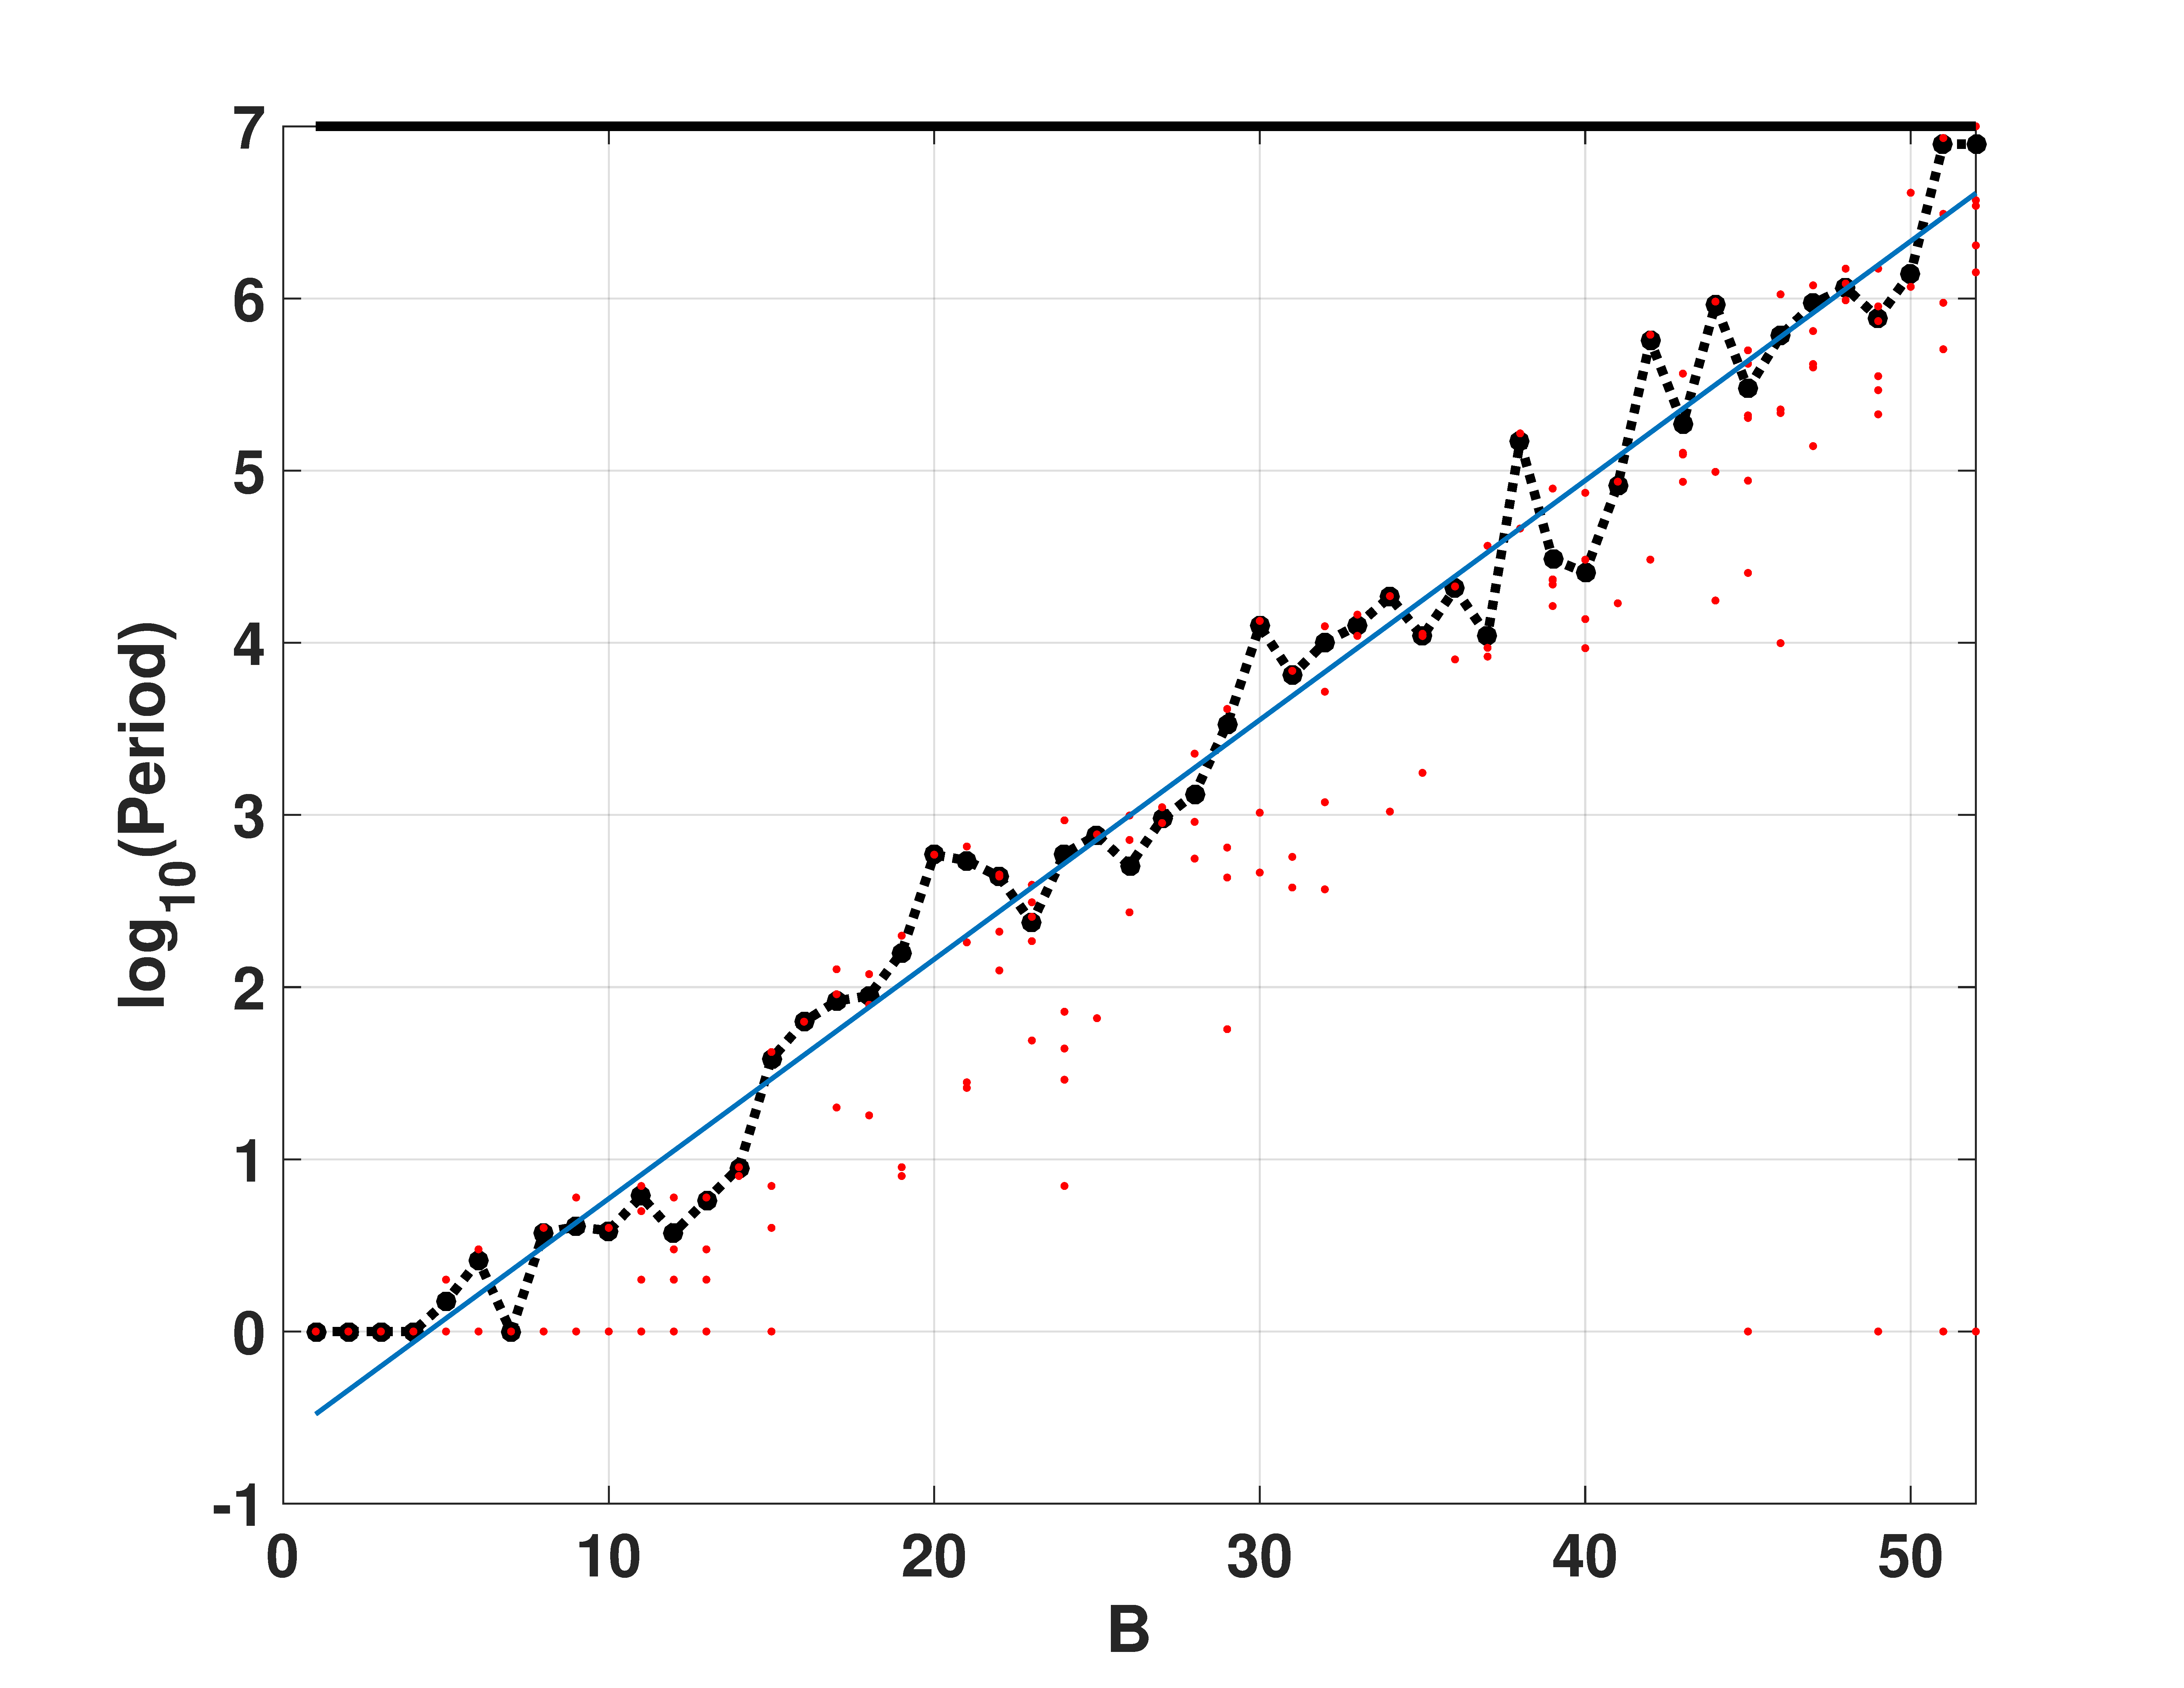
\includegraphics[width=.49\textwidth]{Period_Logistico}
	\caption{Period as function of presition in binary digits} \label{fig:period}
\end{figure}

\begin{table}
	\caption{Period $T$ as a function of $B$ for the maps considered}
	\label{tabla:periodos}
	\begin{tabular}{lll}
		\hline\noalign{\smallskip}
		map & m & b  \\
		\noalign{\smallskip}\hline\noalign{\smallskip}
		TENT&0 & 0 \\
		LOG &0.139 & -0.6188 \\
		SWITCH &0.1462 & -0.5115 \\
		EVEN &0.1447 & -0.7783 \\
		ODD &0.1444 & -0.7683 \\
		\noalign{\smallskip}\hline
	\end{tabular}
\end{table}

Results are compatible for those obtained in \cite{Nagaraj2008}. Switching between maps increase de period $T$ but the skipping procedure decrease it esentially to one half. 

